\subsection{2-D interchange model with fluid neutrals}\label{sec:2D_interchange}

After P.~Tamain~(private communication), the equations for time advance
of respectively electron number density~$n_e$, ``vorticity"~($\nabla \cdot {\bf E}^{+}$),
electron energy~$\mathcal{E}_e$, ion energy~$\mathcal{E}_i$ and 
neutral number density~$n_n$ are respectively
\begin{eqnarray}
& & \partial_t n_e + \nabla \cdot \left( n_e {\bf u}_e \right) = 
S^n_{e} - \frac{n_e}{\tau_{n_e}} \\
& & \partial_t \nabla \cdot {\bf E}^{+} + \nabla \cdot 
\left( \nabla \cdot \left( {\bf u}_i \otimes {\bf E}^{+} \right) 
\right) = \nabla \cdot \left( n_i \left( {\bf u}_{\nabla B i} + 
{\bf u}_{cx} \right) - \frac{1}{{Z_i}} n_e {\bf u}_{\nabla B 
e} \right) \nonumber \\
& & \hspace{5cm} + \frac{1}{{Z_i}} \frac{n_e}{\tau_{n_e}} - 
\frac{n_i}{\tau_{n_i}} + \nabla \cdot \left( {\nu} 
\nabla_\perp \left( \nabla \cdot {\bf E}^{+} \right) 
\right) \\
& & \partial_t \mathcal{E}_e + \nabla \cdot \left( \mathcal{E}_e {\bf u}_e + p_e 
{\bf u}_e \right) = S^{\mathcal{E}}_{e} - \frac{\mathcal{E}_e}{\tau_{Ee}} + Q_{ie} + 
\nabla \cdot \left( {\kappa_{\perp e}} n_e 
\nabla_\perp kT_e \right) \\
& & \partial_t \mathcal{E}_i + \nabla \cdot \left( \mathcal{E}_i {\bf u}_i + p_i 
{\bf u}_i \right) = S^{\mathcal{E}}_{i} - \frac{\mathcal{E}_i}{\tau_{Ei}} - Q_{ie} + 
\nabla \cdot \left( {\kappa_{\perp i}} n_i 
\nabla_\perp kT_i \right) \\
& & \partial_t n_n = S^n_{n} + \nabla \cdot \left( D_n  
\nabla_\perp p_n \right)
\end{eqnarray}
where with the usual notation for species~$\alpha$, pressure~$p_\alpha$,
temperature in energy units~$kT_\alpha$, charge state~$Z_i$,
species mass~$m_\alpha$, electric potential~$\Phi$ and magnetic field~${\bf B}$, 
\begin{eqnarray}
& \mbox{ ion number density} & n_i = n_e \\
& & \mathcal{E}_{\alpha} = \frac{3}{2} p_{\alpha}  = \frac{3}{2} n_{\alpha} kT_{\alpha},\;\; \alpha=i,e \\
& \mbox{ modified electric field} & {\bf E}^{+} = \frac{m_i}{Z_i e B^2} \left( n_i \nabla_\perp 
\Phi + \frac{1}{Z_i e} \nabla_\perp p_i \right) \\
\end{eqnarray}


Perpendicular advection velocities:
\begin{eqnarray}
{\bf u}_e & = & {\bf u}_{E \times B} + {\bf u}_{\nabla B e} + 
{\bf u}_\textrm{diff}\\
{\bf u}_i & = & {\bf u}_{E \times B} + {\bf u}_{\nabla B i} + 
{\bf u}_\textrm{diff} + {\bf u}_{cx}
\end{eqnarray}
with
\begin{eqnarray}
& & {\bf u}_{E \times B} = \frac{\mu_{cx}^2}{1+\mu_{cx}^2} 
\frac{{\bf B} \times \nabla \Phi }{B^2} \\
& & {\bf u}_{\nabla B i} = \frac{\mu_{cx}^2}{1+\mu_{cx}^2} \frac{2 
kT_i}{Z_i e B} \frac{{\bf B} \times \nabla B }{B^2} \\
& & {\bf u}_{\nabla B e} = -\frac{2 kT_e}{e B} \frac{{\bf B} \times 
\nabla B }{B^2} \\
& & {\bf u}_{cx} =  \frac{\mu_{cx}}{1+\mu_{cx}^2} \frac{1}{B} \left( 
-\nabla_\perp \Phi -\frac{1}{Z_i e n_i} \nabla p_i \right) 
\\
& & {\bf u}_\textrm{diff} = - {D_\perp} \nabla n_e
\end{eqnarray}
with the magnetization with respect to charge exchange reactions 
defined as $\mu_{cx}=\omega_{ci}/\nu_{cx}$, $\omega_{ci} = Z_i 
|e| B/m_i$ being the ion cyclotron frequency and $\nu_{cx}=K_{cx} n_n$ 
the charge exchange frequency ($K_{cx} \left( n_i, T_i \right)$ is the 
reaction rate of charge exchange reactions). 

Loss rates can be given several meanings in this kind of model. They 
can be prescribed as parameters, but they can also describe sheath 
losses in which case they have a non-linear dependency with the plasma 
conditions, eg.\ 
\begin{eqnarray}
\tau_{n_e} & = & \frac{L_\|}{c_s}\exp\left(\Lambda_b - \frac{e \Phi}{kT_e}\right) \\
\tau_{n_i} & = & \frac{{L_\|}}{c_s} \\
\tau_{\mathcal{E}_e} & = & \frac{2}{3 {\delta_e}} \tau_{n_e} \\
\tau_{\mathcal{E}_i} & = & \frac{2}{3 {\delta_i}} \tau_{n_i}
\end{eqnarray}
where $c_s = \sqrt{\frac{kT_i + {Z_i} kT_e}{{m_i}}}$ 
is the acoustic velocity and
\begin{equation}
\Lambda_b=-\frac{1}{2} \ln \left[ 0.5 
{\frac{m_e}{m_i}} \left( 1 + \frac{T_i}{T_e} \right)
\right]
\end{equation}
is the sheath potential drop normalized to $T_e$.

The collisional energy equipartition term (from Braginskii) is:
\begin{equation}
Q_{ie} = 3 {\frac{m_e}{m_i}} \frac{n_e}{\tau_e} \left( kT_e - kT_i \right)
\end{equation}
with the electron collision time given by: 
\begin{equation}
\tau_e = \frac{3 \left(2 
\pi \right)^{3/2} \epsilon_0^2 \sqrt{m_e} (kT_e)^{3/2}}{n_i 
{Z_i}^2 e^4 \Lambda}
\end{equation}
and $\Lambda$ is the Coulomb 
logarithm (which has a weak dependence on~$n_e$ and~$T_e$ as indicated in \Sec{coefficient}).

Source terms:
\begin{eqnarray}
S^n_{e} & = & -S^n_{n} = n_e n_n K_i \left( n_e, T_e \right) - n_e^2 
K_r \left( n_e, T_e \right) \\
S^{\mathcal{E}}_{e} & = &  - n_e n_n K_i \left( n_e, T_e \right) \mathcal{E}_i 
\left( T_e \right) - n_e^2 K_r \left( n_e, T_e \right) \frac{3}{2} kT_e 
\\
S^{\mathcal{E}}_{i} & = &  - n_e^2 K_r \left( n_e, T_e \right) \frac{3}{2} kT_i
\end{eqnarray}
where $K_i$ and $K_r$ are the ionization and recombination reaction rates.

Neutral diffusion coefficient:
\begin{equation}
D_n = \frac{1}{m_i \left( n_i K_{cx} ( n_i, T_i ) + n_e K_i ( n_e, T_e ) \right)}
\end{equation}
Other perpendicular diffusion coefficients from Braginskii as
in \Sec{coefficient}.

Boundary conditions:
\begin{itemize}
\item electron density $n_e$: zero flux
\item electron energy $\mathcal{E}_e$: zero flux
\item ion energy $\mathcal{E}_i$: zero flux
\item electrostatic potential $\Phi$: Dirichlet equal to 
average of $\Lambda_b T_e$ along the boundary
\item neutral density $n_n$: incoming flux fixed by integral of 
particle losses in parallel direction (exact redistribution to be 
discussed)
\end{itemize}

\subsection{Coupling to particles}\label{sec:coupart2D}
The only appearance of particle or kinetic effects in the model of \Sec{2D_interchange}
is via the sheath
boundary condition. A more detailed treatment of the sheath uses particle
techniques cf.\ \Sec{sys2-5}, where the different representation is used in
a second overlapping region as indicated in \Fig{pcleadj} taken from
ref~\cite{y1re231}.
\begin{figure}
\centerline{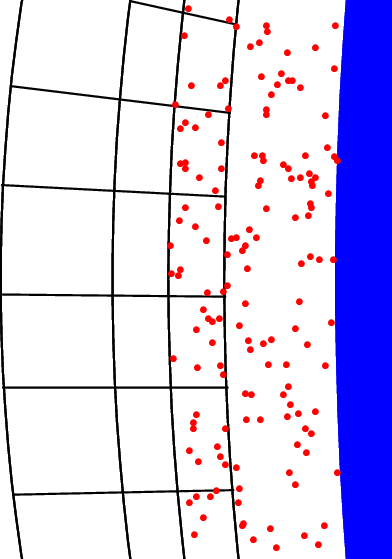
\includegraphics[width=6cm]{../png/pclovm}}
\caption{Handling a plasma sheath adjacent to wall at right.
Plasma has fluid properties discretised using FEM indicated using warped grid,
but in sheath is better represented as particles indicated by dots.\label{fig:pcleadj}} 
\end{figure}


